\documentclass[10pt,a4paper,twocolumn]{scrartcl}
\usepackage[utf8]{inputenc}
\usepackage[english]{babel}
\usepackage[T1]{fontenc}
\usepackage{amsmath}
\usepackage{amsfonts}
\usepackage{amssymb}
\usepackage{graphicx}
\usepackage{setspace}
\usepackage[left=2cm,right=2cm,top=2cm,bottom=2cm]{geometry}

\usepackage{booktabs}

\usepackage{hyperref}

\usepackage{natbib}
\bibliographystyle{alpha}
%\bibliographystyle{spr-chicago}
%\bibpunct[:\,]{(}{)}{;}{}{}{,}

\title{Reception of LGBT in Newspapers}
\author{Magdalena Bönisch \and Till Haubenreißer \and Maximilian Möller}
\publishers{\emph{Universität Leipzig, Introduction to Digital Humanities (Dr. Köntges)}}

\begin{document}
\onehalfspacing

\maketitle

{\footnotesize
\paragraph*{Abstract} Here are 150 to 200 words which constitute our abstract.
}


\section{Introduction}
This is our pretty Introduction.

\section{Workflow \& Implementation}
In the following, the general workflow for analyzing the LGBT reception within newspapers is described. Subsequently, the concrete decisions concerning the implementation are addressed.

\subsection*{Workflow} The overall workflow is shown in Fig.~\ref{fig:workflow}. The upper part reflects the first step of collecting newspaper articles and creating a database. For each term from a predefined list of query terms, an HTTP request to the API of an online newspaper archive is sent. In this work, the Article Search API of the New York Times\footnote{\url{https://developer.nytimes.com/}} has been used as it provides access to articles published since its foundation in 1851 and thus enables an extensive time-dependent analysis. Furthermore, the returned JSON documents contain not only a URL to the actual article but also textual attributes like the lead paragraph and the publication date. The analysis is based on these text fields. Hence, no further call for the complete article is necessary. Since the access to the NYT API is limited per second and per day, the responses are parsed and stored into a MySQL\footnote{\url{https://www.mysql.com/}} database. A relational database allows a quick access to the data along with SQL as a powerful query language for data selection and summarization. By using the database, subsequent analysis is based on the whole corpus independent of the API. Furthermore, the proposed workflow is more flexible with respect to adding data from an additional newspaper archive since its response only has to be mapped to the schema of the database while the analysis module (lower part of the workflow in Fig.~\ref{fig:workflow}) remains unaffected.

\begin{figure}
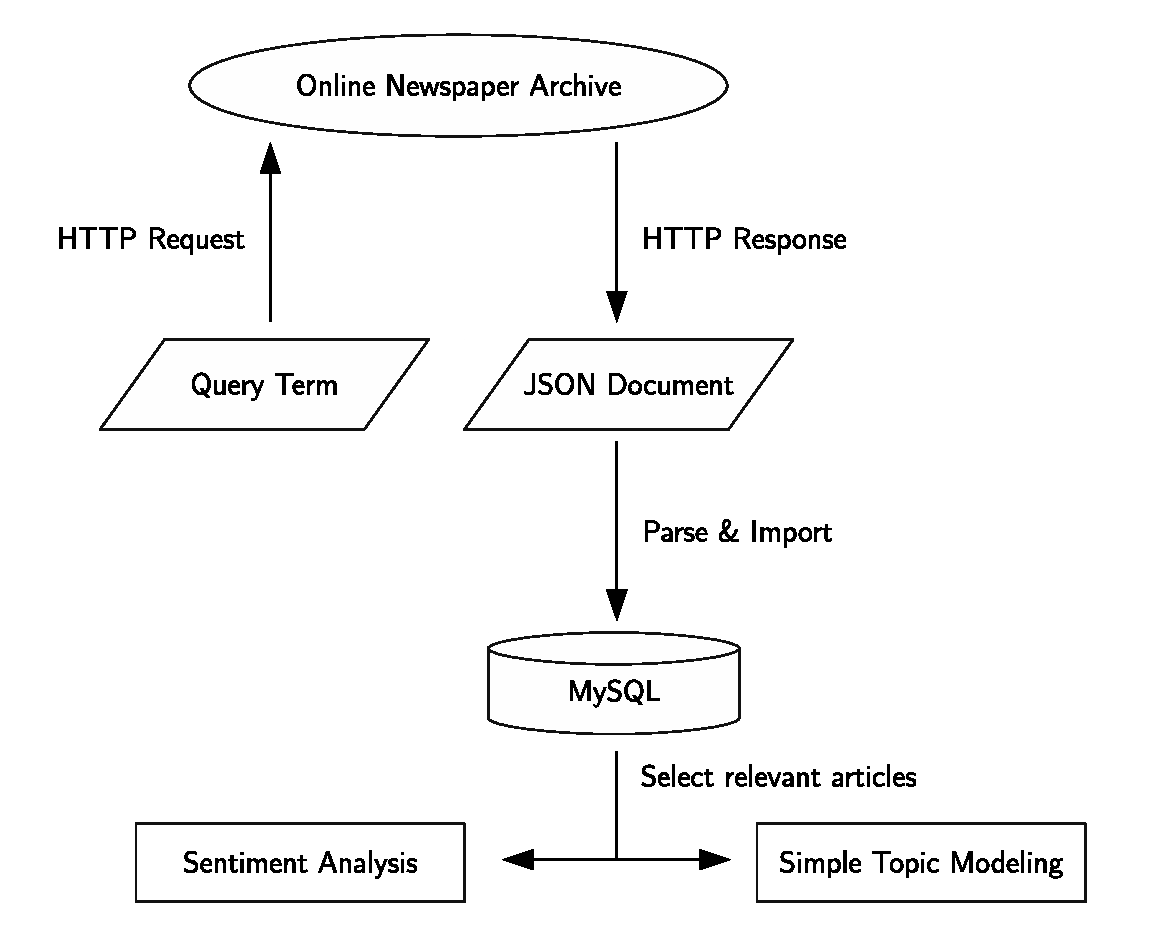
\includegraphics[width=\columnwidth]{figures/workflow_eps}
\caption{Workflow} \label{fig:workflow}
\end{figure}

The analyses are based on two dimensions: query term and time. Thus, the input of the sentiment analysis and the simplified topic modeling approach is a set of lead paragraphs containing the query term and contained in articles published at a certain time. For instance, such an input can be all lead paragraphs from the database which contain the word \textit{homosexual} and which were published in the 1990s.

The sentiment analysis assigns each sentence a vector of sentiment probabilities. We have considered five sentiments: \textit{very negative}, \textit{negative}, \textit{neutral}, \textit{positive}, and \textit{very positive}. For example, the vector \begin{center}
$v_s = \langle 0.2, 0.5, 0.1, 0.1, 0.1\rangle$
\end{center} describes the case that a sentence $s$ has a probability of $20\%$ for having a very negative sentiment, $50\%$ for having a negative sentiment, and $10\%$ for having a neutral, positive, and very positive sentiment, respectively. For the topic modeling, the joint occurrence of a target term together with another word (cooccurrence) is analyzed. Target terms are LGBT-related words, like the query terms.\footnote{The query terms are used for building an LGBT-corpus. But within this corpus it is possible to search for other terms than query terms as well. For instance, \textit{lesbian} is a query term as well as a target term. \textit{gay} is only a target term.} For each cooccurrence, its frequency and its significance is calculated. For instance, the cooccurrence \begin{center}
$c_\text{2010s} = \langle \text{bisexual}, \text{rights}, 31, \text{true}\rangle$
\end{center} means that within the lead paragraphs from 2010 to 2019, \textit{bisexual} and \textit{rights} occurred 31-times in the same paragraph and that this occurrence is significant. By clustering significant cooccurrences, the topics were manually created in order to yield high-quality topics.

\subsection*{Implementation} The whole workflow has been implemented in Java as a Maven\footnote{\url{https://maven.apache.org/}} project. The project is managed on GitHub.\footnote{\url{https://github.com/macksimiljan/lgbt-news}} It consists of one module for collecting and one for analyzing the data. The database is accessed by using the Java Database Connectivity (JDBC) API\footnote{\url{http://www.oracle.com/technetwork/java/javase/jdbc/index.html}}.

\paragraph*{Collecting Module} The used query terms are \textit{bisexual}, \textit{gay community}, \textit{homosexual}, \textit{lesbian}, \textit{transgender}, and \textit{transsexual}. However, the term \textit{gay} was not considered as a query term because it appeared too often in non-LGBT-related contexts, as a given name or surname, for instance. In order to obey the time limit of the NYT API, only one request per second was sent. Almost all requests ($95.4\%$) were successful. They returned a non-empty JSON object which was then inserted into the database. Failures of requests were due to denied access to the archive (HTTP 403) or gateway time-outs (HTTP 504). Because such failures were very rare, failed requests were not sent for a second time. All in all, the built corpus consists of $44,485$ articles, $93,7\%$ of which contain a non-empty lead paragraph on which the analyses are based.

The database models the mapping of query terms and keywords to articles. Keywords represent additional information on the articles such as associated persons, organizations, or geographical information. Approximately $75\%$ of all articles have at least one keyword. Moreover, an article has a URL which points to its HTML representation in two-thirds of the cases; otherwise the article is only accessible as a PDF document.\footnote{Older articles are archived as PDF not as HTML.} Further attributes are the publication date, the actual text type (for instance, article, interview, or biography), the headline, an abstract, the lead paragraph, and a snippet. Since the headline is very short, the abstract is missing for $62\%$ of the articles, and the snippet is mostly the same as the lead paragraph, the analysis is based on the lead paragraph. For the body of the article, the HTML representation of the article would have had to be requested and parsed.

\paragraph*{Analysis Module} Essentially, the analysis module of the Maven project comprises the sentiment and the topic model package. They both rely on the sentence extraction task. For a certain target term and a certain publication date, this task selects windows of sentences from the paragraphs in the database. Given a window size of 2, for instance, in addition to the sentence containing the target term, the two directly preceding as well the two directly succeeding sentences are extracted.\footnote{For the given corpus, a window size greater than 4 will have no difference to a smaller size since the paragraphs consists only of a few sentences. For instance, not more than 40\% of the paragraphs consists of two or more sentences.} For the sentiment analysis, we have chosen a window size of 0, i.e. only the containing sentence, and for the topic modeling a size of 1.  Both analyses depend on the natural language processing library Stanford CoreNLP\footnote{\url{http://stanfordnlp.github.io/CoreNLP/}}. This library contains annotators for tokenization, sentence splitting, part-of-speech tagging, and sentiment analysis. Since the sentiment annotator is based on the sentence structure, it is expected that it returns better results than approaches which only count the occurrences of particular negatively or positively connotated words or phrases while ignoring their syntactic context \citep{Socher+al:2013}. However, determining the sentence sentiment is a very time consuming operation. Therefore, we have chosen the minimal window size.

The simplified topic modeling approach consists of three steps: preprocessing, cooccurrence counting, and the statistical evaluation. The preprocessing is executed for the corpus only once. For all paragraphs, the contained words and their number of occurrence are determined. Stop words and numbers are excluded from this word statistics. The stop word list is based on \citep[p.533]{Manning+Schuetze:2003} whereas numbers are recognized by a regular expression. After having created the word statistics, it is possible to define the list of context words. A context word is a meaningful word which cooccurs with a target term. A word is assumed to be meaningful if it is not a stop word or a number and has a minimum frequency of 3. The frequency condition enforces that words being typographical errors are excluded from the analysis. After preprocessing, the word statistics consists of approximately $66\cdot 10^3$ word types and $1.2 \cdot 10^6$ word tokens.\footnote{Since we followed a simple approach, we did not run a lemmatizer. For comparison, the Oxford Dictionary counts about $200 \cdot 10^3$ (lemmatized) word types (inclusive stop words) in the English language \citep{Oxford}.}  $43.4\%$ of all words occur only once or twice. Thus, there are approximately $29\cdot 10^3$ context words.

In the next step, all cooccurences of a target word $w_\text{target}$ with one of the $n$ context words are counted in the paragraphs containing $w_\text{target}$ and published in a certain time span $t$. To yield the cooccurrences and their number, these paragraphs were tokenized and cleansed by removing all non-context words from the sentences and transforming the remaining words to lower case. For instance, the sentences \begin{center}\textit{The president argues for gay rights. He is tolerant.}\end{center} is mapped to \begin{center}\textit{president argues gay rights tolerant}\end{center} This sequence of words is used to built a context vector $v_t(w_\text{target}) = \langle c_1, c_2, \ldots, c_n\rangle$ for each $w_\text{target}$ and $t$ such that $c_i$ represents the (absolute) frequency of the cooccurrence of $w_\text{target}$ with the context word at list position $i$. Because cooccurrence is not a reflexive relation between two words, $c_i = 0$ if the context word at position $i$ equals $w_\text{target}$. In the example, assume that the list of context words $L$ consists of six words: \begin{center}$L =  [\text{argues, gay, president, rights, tolerant, usa}]$\end{center} Depending on the chosen maximum distance $d_\text{max}$, the context vector $v_t(\text{gay})$ for the target word \textit{gay} is built. Let $d_\text{max}$ be 2, then there can be not more than $d_\text{max} - 1 = 2 - 1 = 1$ word between the target word and its cooccurrence partner. This yields the context vector \begin{center}$v_t^1(\text{gay}) = \langle 1, 0, 1, 1, 1, 0\rangle$\end{center} because every word except for \textit{usa} cooccurs with \textit{gay} exactly once. For $d_\text{max} = 1$, only the direct neighbors of \textit{gay} are considered resulting in the context vector \begin{center}$v_t^2(\text{gay}) = \langle 1, 0, 0, 1, 0, 0\rangle$.\end{center} Studies suggest that the average sentence length in written prose is between 20 and 25 tokens, for instance \citep{Sichel:1974}. The maximum distance $d_\text{max}$ is not sentence-sensitive, i.e., it ignores sentence boundaries. Nevertheless, as the paragraphs are only a few sentences, there is a maximum distance $d'_\text{max}$ such that for all distances greater than $d'_\text{max}$ the number of cooccurrences is the same. Fig.~\ref{fig:distance} shows this for the count of cooccurrences with \textit{gay} in the 2010s. The number of all cooccurrences as well as the number of significant cooccurrences converge to 7650 and to 2300, respectively. These values are reached for a maximum distance greater than 56 (not shown in the figure). Tests with further target words lead to similar results. However, the smaller the maximum distance, the more semantically connected the words of the cooccurrence are expected to be. Choosing a great distance, the cooccurrences can connect words which are probably in different sentences. Since the sentence boundary is a semantic boundary as well (each sentence represents a logical statement on its own), a great maximum distance results in cooccurrences which might include words that should not be interpreted as being semantically connected. Thus, we run the program with a maximum distance of 6 and of 14 for all target terms and times. For  $d_\text{max} = 6$ ($d_\text{max} = 14$), approximately $67\%$ ($85\%$) of all cooccurrences and $40\%$ ($67\%$) of all significant cooccurrences are detected. 


\begin{figure}
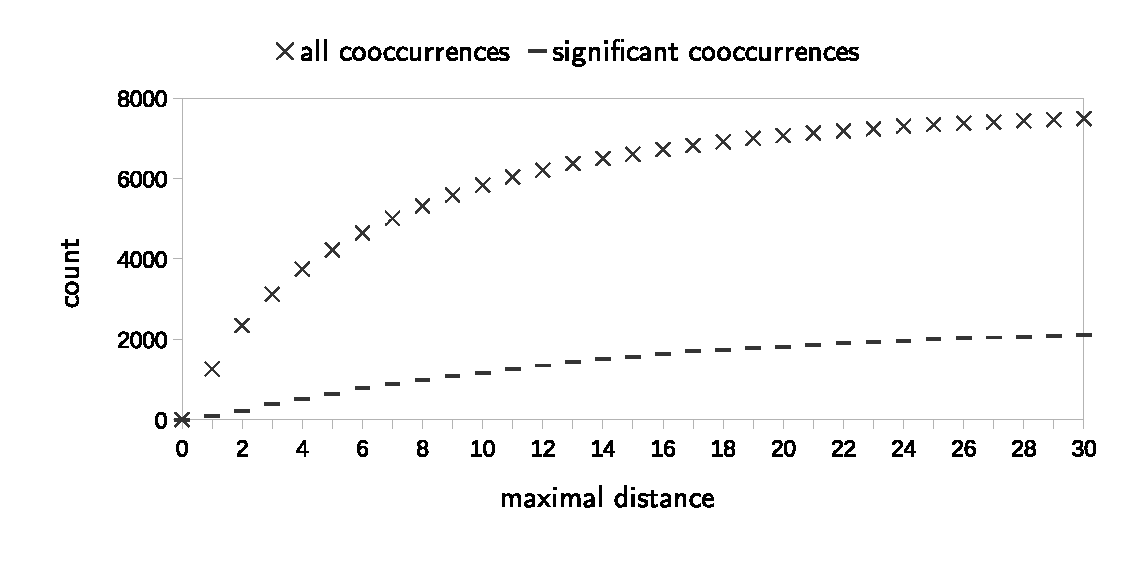
\includegraphics[width=\columnwidth]{figures/distance_eps}
\caption{Convergence of the number of cooccurrences.} \label{fig:distance}
\end{figure}

The last step is the calculation of significant cooccurrences. Following \citep{Bordag2008, Manning+Schuetze:2003}, three significance measures were implemented: mutual information, log-likelihood, and t-score. For some test data, the t-score yields the best results. Let $n$ be the number of context words, $n_\text{t}$ and $n_\text{c}$ the number of occurrences of the target term and of a context word, respectively, and $n_{\text{t}\text{c}}$ the count of the cooccurrence of $w_\text{target}$ and $w_\text{context}$, then the t-score is defined according to Eq.~\ref{eq_tscore}.

\begin{equation}
\text{t}(w_\text{target}, w_\text{context}) = \frac{n_{\text{t}\text{c}} - \dfrac{n_\text{t} \cdot n_\text{c}}{n^2}}{\sqrt{n_{\text{t}\text{c}}}} \label{eq_tscore}
\end{equation}

 Consequently, a cooccurrence is defined as significant if it passes the t-test for $p = 0.005$. Additionally, all cooccurrences were selected occurring more often than on average in order to get further hints for topics. 



\section{Underlying Data}

Choosing the underlying data and retrieving it correctly was a crucial part of our work. Not only we had to (choose) terms that are most used in an LGBT context but also we had to filter the content for relevant articles in our case. There are a lot of terms but not all of them are useful for analysis. In the end we came up with 6 useful terms that delivered enough data to be relevant. These are: \textit{bisexual}, \textit{gay community}, \textit{homosexual}, \textit{lesbian}, \textit{transgender} and \textit{transsexual} making in sum $44,485$ articles and a mean of $95.38\%$ of all articles with these search terms in the NYT database. 

Why did we choose those words as our data foundation? Firstly they are diverse. They cover a wide variety of alternative gender models without going to much into detail. Secondly they are very prominent. As already said if there aren't enough articles the relevance decreases. Thirdly they cover all timespans researchable via the API, the NYT was founded in 1851. Some of the terms were used very early while others gained importance just in the last time. The number of articles per decade for a given query term is shown in Fig.~\ref{fig:bisexual}, Fig.~\ref{fig:gayCommunity}, Fig.~\ref{fig:homosexual}, Fig.~\ref{fig:lesbian}, Fig.~\ref{fig:transgender}, and Fig.~\ref{fig:transsexual}.


\begin{figure}
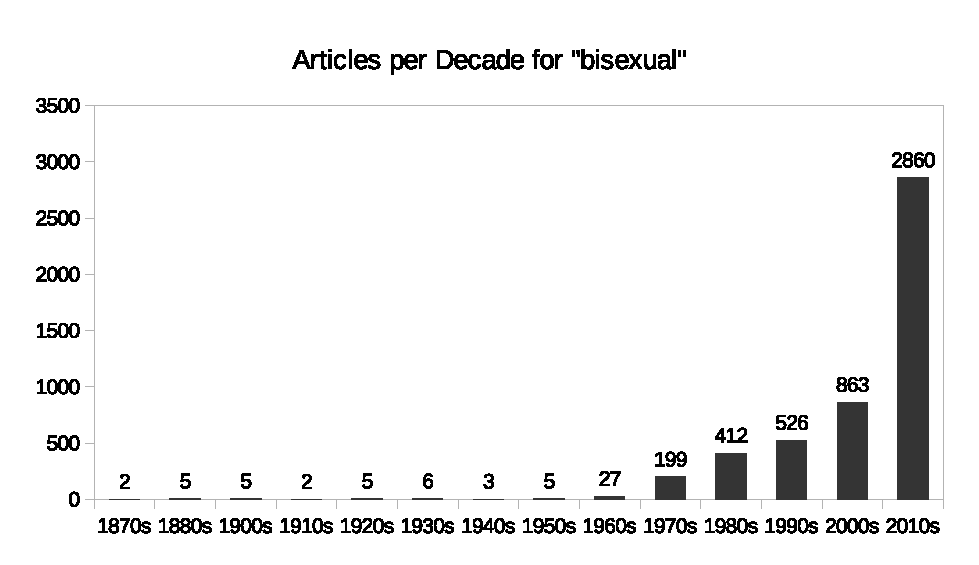
\includegraphics[width=\columnwidth]{figures/bisexual_decade}
\caption{Number of articles for \textit{bisexual}.} \label{fig:bisexual}
\end{figure}

\begin{figure}
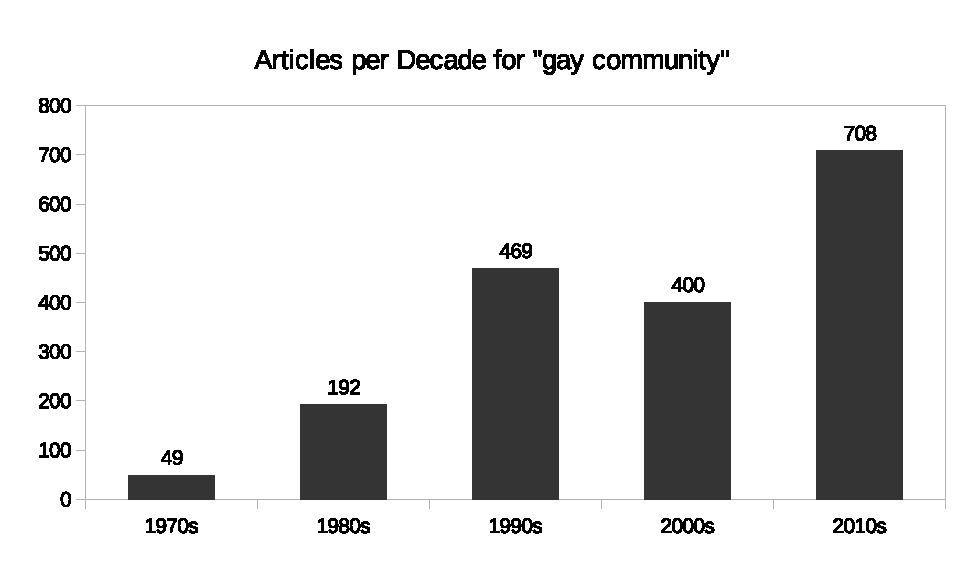
\includegraphics[width=\columnwidth]{figures/gayCommunity_decade}
\caption{Number of articles for \textit{gay community}.} \label{fig:gayCommunity}
\end{figure}

\begin{figure}
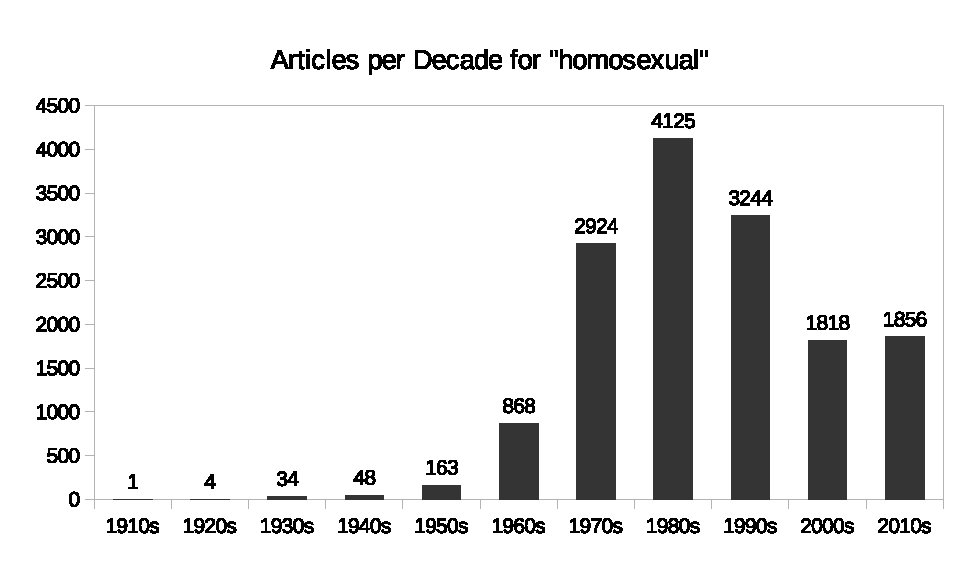
\includegraphics[width=\columnwidth]{figures/homosexual_decade}
\caption{Number of articles for \textit{homosexual}.} \label{fig:homosexual}
\end{figure}

\begin{figure}
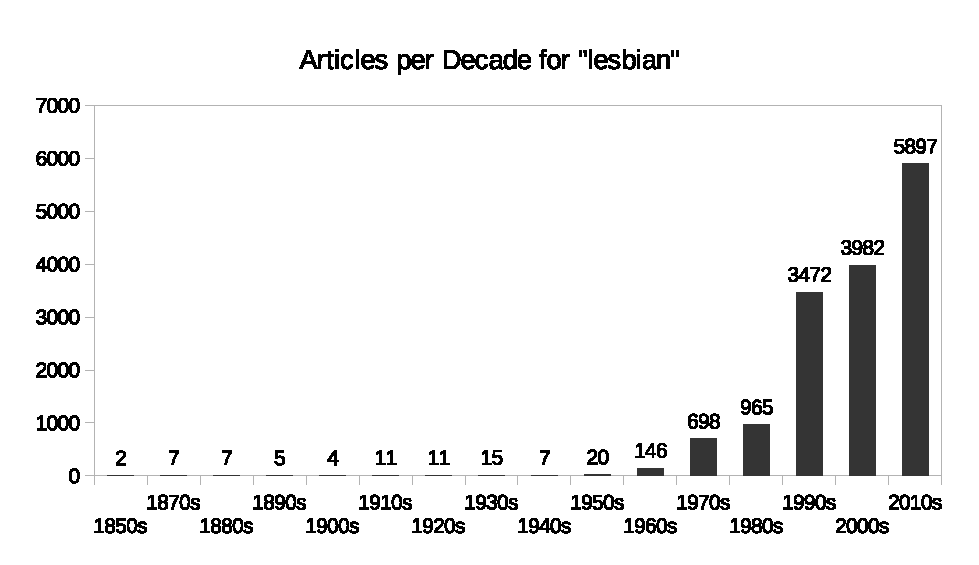
\includegraphics[width=\columnwidth]{figures/lesbian_decade}
\caption{Number of articles for \textit{lesbian}.} \label{fig:lesbian}
\end{figure}

\begin{figure}
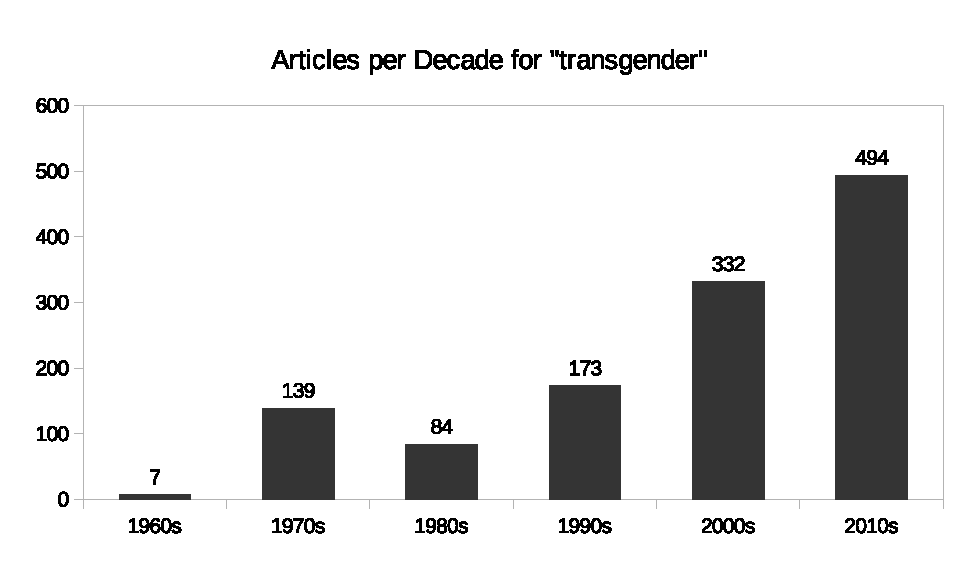
\includegraphics[width=\columnwidth]{figures/transgender_decade}
\caption{Number of articles for \textit{transgender}.} \label{fig:transgender}
\end{figure}

\begin{figure}
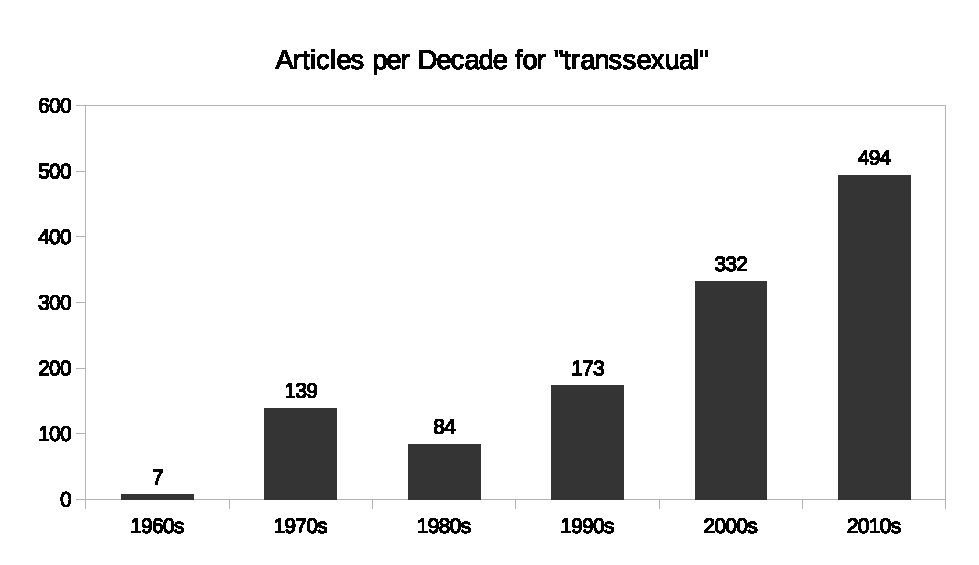
\includegraphics[width=\columnwidth]{figures/transsexual_decade}
\caption{Number of articles for \textit{transsexual}.} \label{fig:transsexual}
\end{figure}


Why didn't we choose other words that are even more prominent for example \textit{gay}? This has several reasons. Let's stay with the word \textit{gay}. It doesn't have an exclusive meaning just in LGBT context. It also means \textit{happy} meaning we would have gotten lots of articles that have nothing to do with our research topic because it was used in the sense of \textit{being happy}. Another reason is, that gay is also a quit common name or part of a name. 
There are a lot of other terms we didn't use due to reasons like not enough relevance, usage in specific context and or not given researchability. 

One thing we thought about analyzing but decided against eventually was a visualization of geographical information. Only 37\% of all articles have an assigned geographical location. Thus, we doubted the relevance of such a visualization.

So we have a lot of articles but that's just one part. The other part is sentiment analysis and topic modeling to really get something out of the texts. For sentiment analysis, we focused on the 1980s and 2010s because for both decades have many articles and we wanted to compare two times which we expected to have very different reports on LGBT. An extended sentiment analysis for other decades would have gone beyond the scope of this work.

The analyses are based on the \textit{lead paragraph} attribute of each article. 94\% of the articles have such a paragraph. Nevertheless, it is not necessarily the case that a lead paragraph assigned to a certain query term actually contains this query term. For instance, although there are $4,920$ `bisexual' articles in the database, only 570 of these articles have a lead paragraph containing \textit{bisexual}. Nevertheless, there are 1495 lead paragraphs containing \textit{bisexual} in the whole database. The difference emerges from the fact that the NYT API does not search within the lead paragraph but only in the headline, byline and body. As our textual analyses are based on the lead paragraph, the count of target terms in all paragraphs in the database is shown in Tab.~\ref{tab:dataBasis}.

Because on target word can occur in more than one lead paragraph, paragraph duplicates are expected. Within the database, 28\% of all lead paragraphs occur more than once. Duplicates are eliminated during selection of paragraphs from the database.

\begin{table}
\centering
\caption{Size of the data basis.} \label{tab:dataBasis}
\begin{tabular}{lrr}
\toprule
term	 & \#articles & \#paragraphs\\
\midrule
bisexual &  $4,920$ & $1,495$\\
gay			& $-$ & $10,392$\\
gay community & $1,818$ & 377\\
homosexual  & $15,086$ & $5,263$\\
lesbian & $15,249$ & $5,086$\\
queer  & $-$ & 162\\
transgender  & $6,138$ & $2,973$\\
transsexual  & $1,229$ & 279\\
\bottomrule
\end{tabular}
\end{table}

Finally, the created corpus has been compared with the Google Books corpus accessed by the Ngram Viewer.\footnote{\url{https://books.google.com/ngrams}} Fig.~\ref{fig:google} shows the relative frequency for LGBT-related terms in American English books. The upper diagram contains our query terms while the lower one visualizes the occurrence of other LGBT terms. Very prominent is the maximum of \textit{lesbian} (red line) in the late 90s. A closer look at our corpus reveals that there is a similar maximum for \textit{lesbian} but some years earlier. Since newspaper articles are assumed to reflect events more immediately than books, we concluded that it is the same maximum. However, the decrease of \textit{bisexual}, \textit{homosexual}, and \textit{lesbian} since the late 90s, can be only confirmed for \textit{homosexual} in our corpus. The steady increase of \textit{transgender} and \textit{transsexual} is attested in both corpora. The lower diagram shows the frequency of \textit{gay} and \textit{queer}. The characteristic of both terms is that they are present in the literature long before the upper terms occur. Furthermore, as soon as the upper terms emerged, the frequency of \textit{gay} and \textit{queer} decreased while an increase can be observed since the 90s. The hypothesis is that these terms changed their meaning in an infrequent phase from 1940 to 1990 and since that they have been frequently used as LGBT terms.

\begin{figure*}
\centering
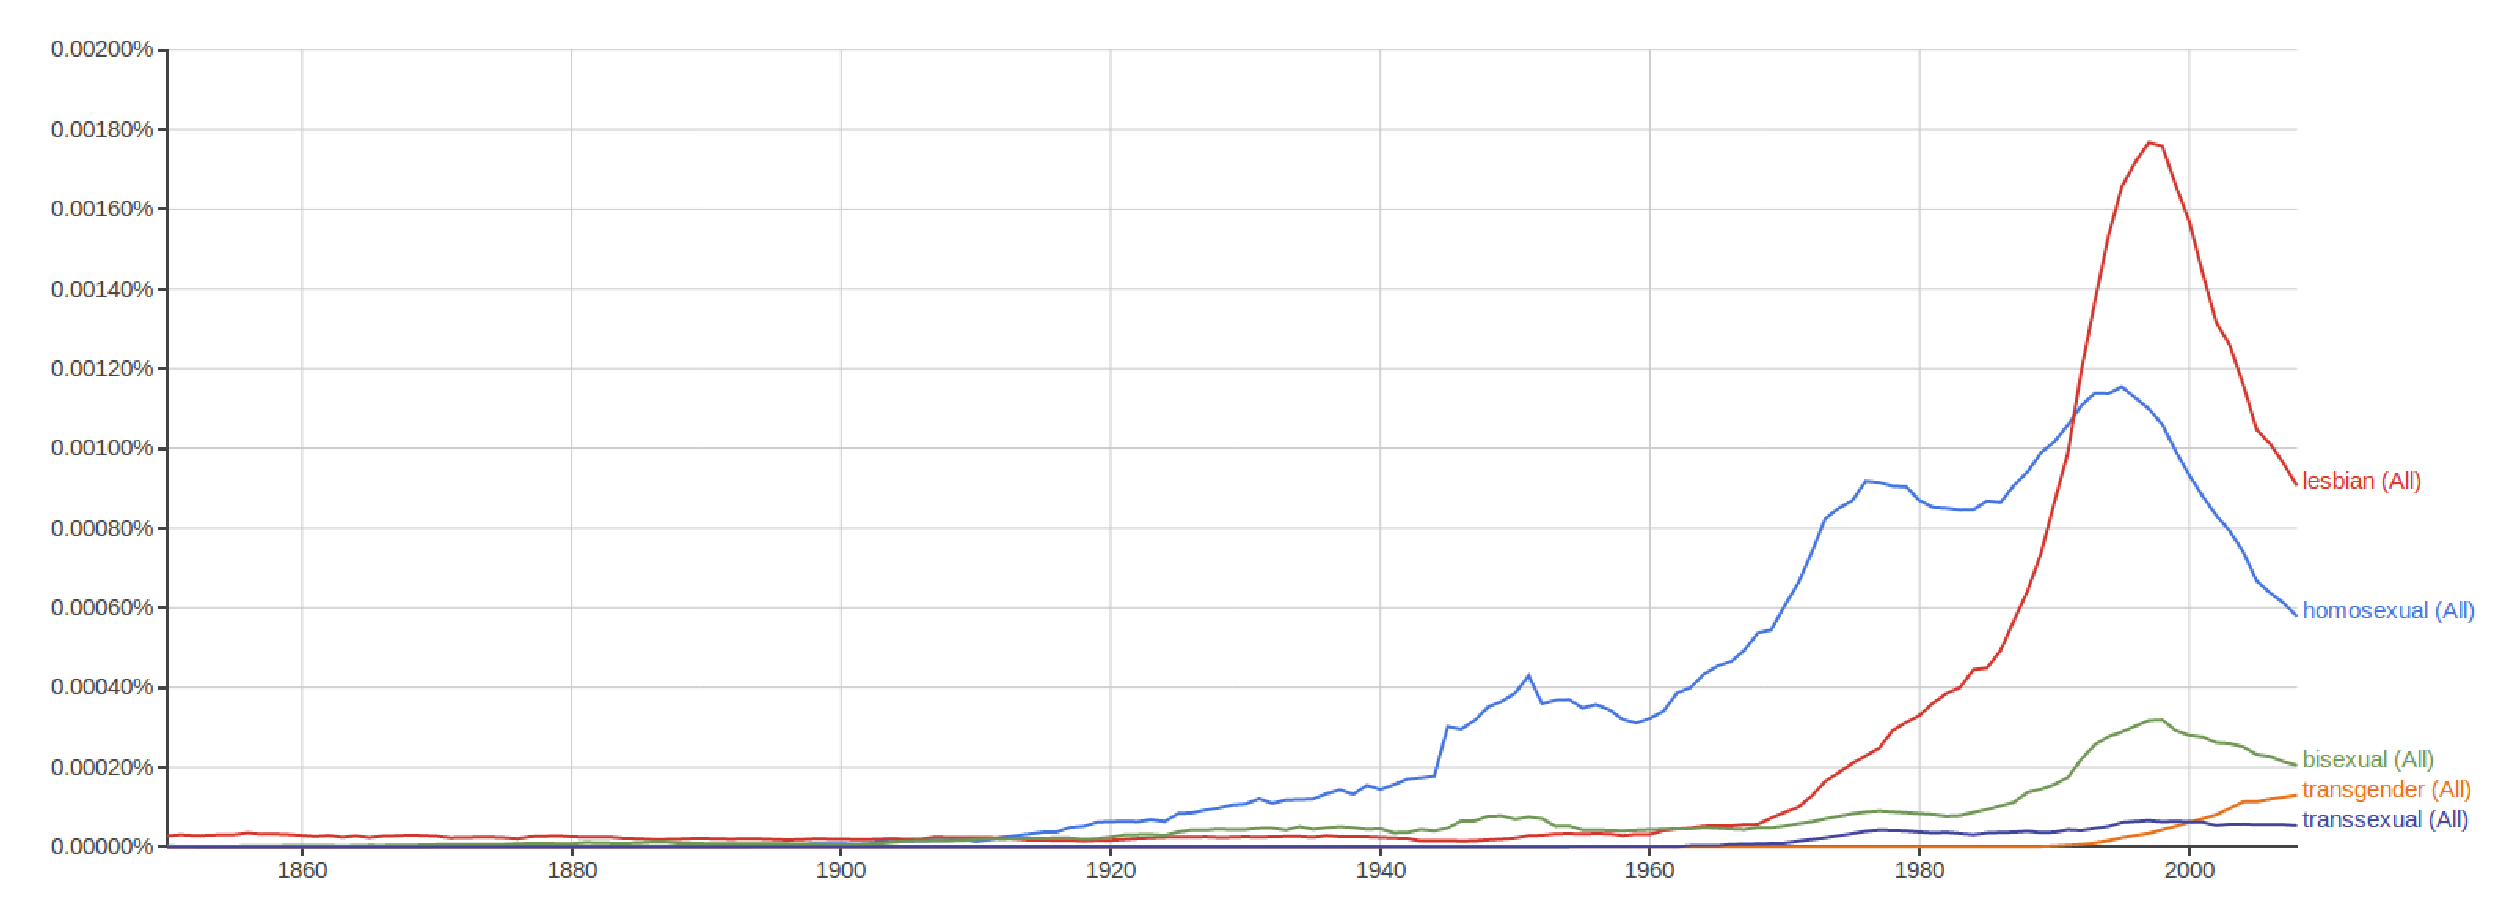
\includegraphics[width=\textwidth]{figures/google_queryterms}

\vspace*{1cm}

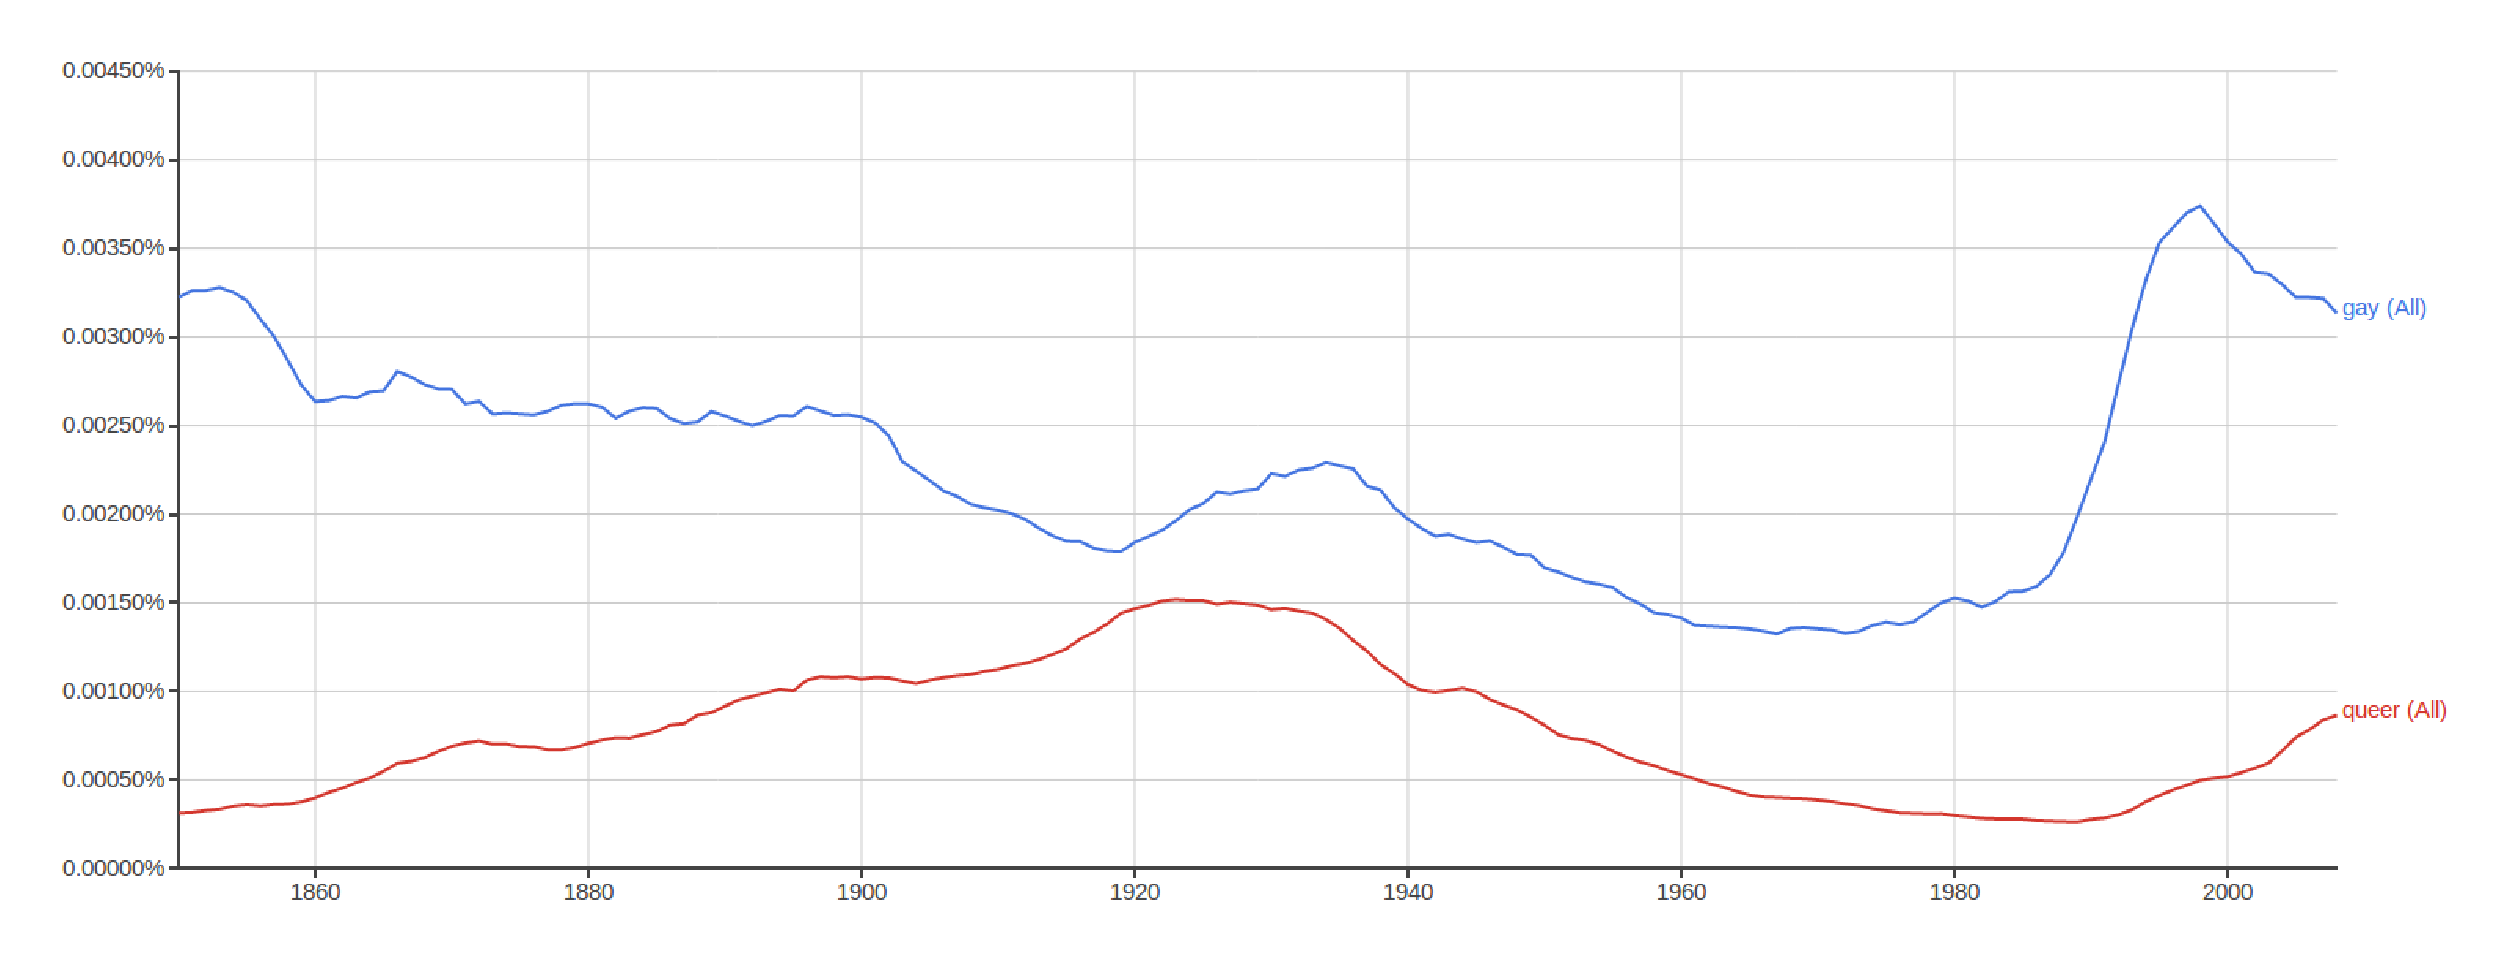
\includegraphics[width=\textwidth]{figures/google_others}
\caption{Google Books Ngram Viewer: LGBT-related terms.} \label{fig:google}
\end{figure*}



\section{Results}

\subsection{Sentiment Analysis}

For the sentiment analysis, we compared the sentiments of sentences containing a target word from early newspaper articles (1980s) with ones from current articles (2010s). Furthermore, the sentiment results among the target words were compared. All in all, there were no significant differences within these conditions. On average, 85\% of all sentences are assigned the sentiment \textit{negative}. \textit{very positive} is determined to less than $0.1\%$ of all input sentences of a sentiment analysis. The frequencies of the other sentiments are in the range of 2\% to 8\%. All standard deviations are smaller than $1.5\%$ percent points. There are two explanations for the minimal differences between the conditions. First, the sentiment distribution mainly depends on the genre, i.e., all newspaper articles are written in the same manner. Each article reports the events objectively and with no significant attitude of the author. The mostly negative sentiments are a side-effect of the newspaper ductus. Second, there has been (and still is) a negative reporting for all LGBT news.

To test both explanations, further articles were extracted from the NYT article archive as a baseline for expected positive sentiments. These articles were football news as we assumed that reporting on football is positive. The distributions of sentiments over sentences for LGBT terms and the football baseline are shown in Fig.~\ref{fig:sentiment1}. The \textit{football} data show indeed more positive sentiments than LGBT news. However, about 70\% of all sentences\footnote{For \textit{football}, the input of the sentiment analysis comprises 125 sentences.} have a still a negative sentiment. Thus, we have concluded that negative sentiments are very likely due to the newspaper genre.

\begin{figure}
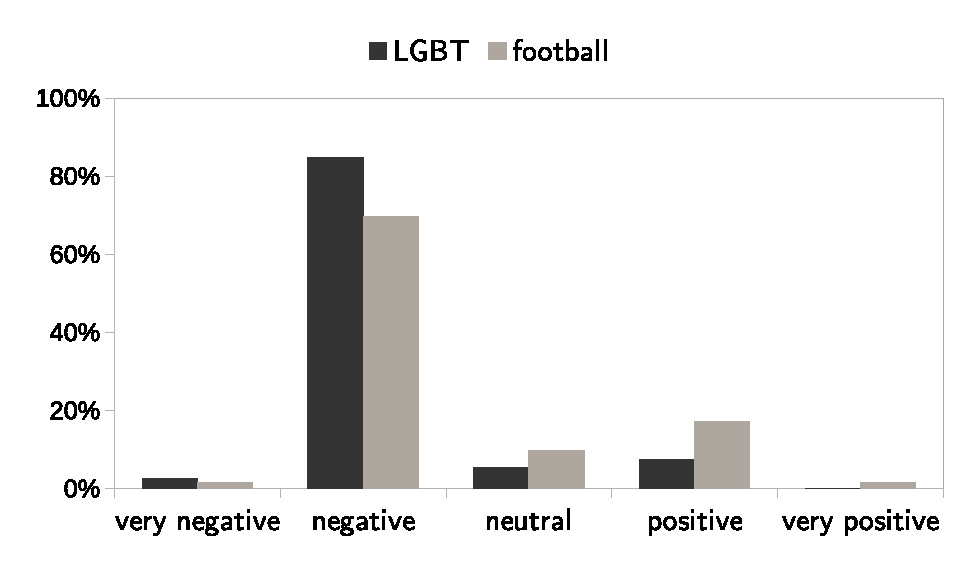
\includegraphics[width=\columnwidth]{figures/sentiment1}
\caption{Frequency of sentiments.}\label{fig:sentiment1}
\end{figure} 

It is important to bring to mind that the output of the sentiment analysis is not a sentiment category in the first place. Rather, an vector of probabilities is returned.  Hence, it might be possible that the competition between sentiments was very close. For the sentiment vector $v_{s_1} = \langle 0.0, 0.46, 0.1, 0.44, 0.0\rangle$, for example, the decision for \textit{negative} and against \textit{positive} is very close since the difference in the probabilities is marginal. However, for the vector $v_{s_2} = \langle 0.0, 0.8, 0.1, 0.1, 0.0\rangle$ it is clear that the sentence $s_2$ has a negative sentiment.

But also on the underlying probability level, the results are equal for all conditions. The averaged probabilities are summarized in Tab.~\ref{tab:prob}. For the articles from the 1980s (2010s), the standard deviation is less than $1.3$ ($1.5$) percent points. Since the expected probability of each sentiment is $^{100\%}/_{5} = 20\%$  for a random distribution, a probability for \textit{negative} greater than $40\%$ can be seen as a clear result. Nevertheless, there is still a certain probability of about $20\%$ that such sentences are \textit{neutral} instead of \textit{negative}. A similar pattern emerges for \textit{football}.

\begin{table*}
\centering
\caption{Average sentiment probabilities.} \label{tab:prob}
\begin{tabular}{lccccc}
\toprule
data & very negative & negative & neutral & positive & very positive\\
\midrule
LGBT, 1980s & 16.9\% & 51.0\% & 20.5\% & 8.7\% & 2.8\%\\
LGBT, 2010s & 16.5\% & 51.9\% & 19.8\% & 8.8\% & 3.0\%\\
football &  13.6\% & 44.8\% & 21.3\% & 14.4\% & 5.9\%\\
\bottomrule
\end{tabular}
\end{table*}

To summarize, the sentiment analysis showed no differences between target terms or different times. A detailed evaluation of the precision of the sentiments is presented in the discussion.

\subsection{Simple Topic Modeling}
This is our great topic modeling.

\section{Discussion}
This is our insightful discussion.

\subsection{Implementation Issues}
In order to compare the reception of LGBT-related terms in different newspapers, it is necessary to integrate further newspaper articles into the database. Especially for The Guardian\footnote{\url{http://open-platform.theguardian.com/}}, the integration into the database is no problem since the Guardian API returns less information than the NYT API, e.g. no publication date or lead paragraph. At the same time, this is a problem because the only information is the web URL to the article. Thus, in order to get the publication date and textual information, the workflow has to be extended by a further request for receiving the HTML page of the full article as well as by a parser for extracting relevant information from this HTML document. As soon as such an extension has been implemented, it can be used to get the full article also from the NYT archive. The full article body would enable a more comprehensive topic modeling. Attention should be paid that the Guardian API provides only access to publications dating back to 1999.

A general problem with the newspaper archive APIs is that the access is limited. Assume that there are $150 \cdot 10^3$ articles for a certain query term as it is the case for \textit{gay} in the NYT archive. Since the NYT API allows requesting only $10\cdot 10^3$ articles per day, collecting the whole result set would take 15 days. The same amount of articles is no problem for the Guardian API where $250\cdot 10^3$ articles can be requested per day.\footnote{The Guardian allows $5\cdot 10^3$ calls per day and a maximum amount of 50 articles per call.} Additionally, only the first 1200 articles can be addressed within requests to the NYT API. Consequently, in order to get all articles, each call should not return more results than this number. In our workflow, the publication date was restricted in order to obtain an appropriate result set size.

In the present paper, sentences were treated differently. On the one hand, sentences were assumed to be important semantic units. Thus, the sentiment analysis was only executed for the sentence containing the target word. On the other hand, sentence boundaries were ignored for the simple topic model. The underlying argument is that in order to extract the topic in which the target word occurs, it is not only worthwhile to look at the sentence but to consider the context of that sentence as well. Nevertheless, this argument can be also applied to the sentiment analysis. Thus, increasing the window size for sentiment analysis should be evaluated in further investigations. Then, the information on coocuccrences and sentiments can be extended by the distance from the target word. Cooccurrences along a great distance may be less informative as direct neighbors. In addition, the sentiment of the sentence containing the target word has a larger weight then the one of other sentences. Then, an outstanding issue is the aggregation function when combining the results of different distances.

The evaluation of the cooccurrences has revealed that there are still a lot of `un-meaningful' words, for instance \textit{only}, \textit{some}, \textit{recent} but also \textit{people} and \textit{group}. Such words make it harder to evaluate cooccurrences. Thus, the stop word list should be expanded by \textit{only} and others. Alternatively, a part-of-speech tagger can be used instead of the stop word list. Then, cooccurrences are only considered for particular part-of-speech, e.g. for nouns and verbs. Furthermore, too generic words (\textit{people}) should be excluded from the context words as well. 


 
// TODO: only cooccurrences of sentences? define max distance dynamically?
// TODO: count the distance from coWord to the targetWord

\subsection{Content Issues}




\subsection{Future Work}

\section{Conclusion}
This is our awesome conclusion.

{\footnotesize \bibliography{lit}}

\onecolumn

\newpage

\section*{Who did What?}

\renewcommand{\arraystretch}{1.5}
\begin{center}
\begin{tabular}{lccc}
\toprule
Task		& M. Bönisch & T. Haubenreißer & M. Möller\\
\midrule
general decisions & $\checkmark$ & $\checkmark$ & $\checkmark$\\
programming & & & $\checkmark$\\
basic data analysis  & & & $\checkmark$\\
diagram creation  & & $\checkmark$ &\\
background recherche & $\checkmark$ & $\checkmark$ & \\
evaluation of sentiment & $\checkmark$ & & $\checkmark$\\
topic evaluation & $\checkmark$ & $\checkmark$ & $\checkmark$\\
introduction text & $\checkmark$ & & \\
workflow \& implementation text & & & $\checkmark$\\
underlying data text & & $\checkmark$ &\\
sentiment results text & & & $\checkmark$\\
homos./bis. topic results text & $\checkmark$ & & \\
lesbian topic results text & & $\checkmark$ & \\
trans*, queer results text & & & $\checkmark$\\
technical discussion text & & & $\checkmark$\\
content discussion text & $\checkmark$ & &\\
future work text\\
conclusion text & & & $\checkmark$\\
typesetting  & & & $\checkmark$\\
\bottomrule
\end{tabular}
\end{center}
\renewcommand{\arraystretch}{1}

\end{document}